%
% Acta Acustica united with Acustica -- Instructions for Authors, 2017-03-01
%
\documentclass[twocolumn]{article}

%%%%%%%%%%%%%%%%%%%%%%%%%%%%%%%%%%%%%%%%%%%%%%%
%% Comment / uncomment for one or two column(s) fomat
%\documentclass{article}

% \usepackage[modulo,switch]{lineno}
% \modulolinenumbers[1]
%%%%%%%%%%%%%%%%%%%%%%%%%%%%%%%%%%%%%%%%%%%%%%%
%% Comment / uncomment for showing line numbers
%  \linenumbers

\usepackage[utf8]{inputenc}
\usepackage{amsmath}
\usepackage{amssymb}
\usepackage{graphicx}

\makeatletter\@ifundefined{date}{}{\date{}}
\makeatother

\markright{\hfill Kergomard {\em et al.}, p.\ }
\pagestyle{myheadings}

\paperheight297mm \paperwidth210mm
\textwidth170mm  \textheight245mm  \oddsidemargin 20mm
\evensidemargin\oddsidemargin \hoffset-22.4mm \voffset-28.4mm
\topmargin0pt \headheight20mm \headsep4mm \topskip0mm
\footskip17.5mm \columnsep7mm \arraycolsep2pt \parindent10pt
\renewcommand{\abstractname}{Summary} 

\begin{document}

\title{Instruction for Authors}

\author{Jean Kergomard$^{1)}$, Thierry Scotti$^{1)}$, Johann Wempen$^{2)}$ \\
$^{1)}$ LMA, CNRS, UPR 7051, Aix-Marseille Univ, Centrale Marseille,\\
   13453 Marseille Cedex 13, France. AAA@lma.cnrs-mrs.fr\\
$^{2)}$ Daucherstr. 98, 85053 Ingolstadt, Germany.}

\maketitle\thispagestyle{empty}

\begin{abstract}
Instead of providing a classic template to be filled in by authors, we
decided that it would be more useful to present with these Instructions
for Authors an example that makes it easy to build \LaTeX{} source files
designed for the review process of Acta Acustica united with Acustica.
The .tex source file of the required format can be downloaded from the
Acta Acustica united with Acustica webpage. To ensure the submission
process as fast as possible, attention of the authors is paid on the
style, design and format of figures that will be submitted (see
$\S$\ref{style}): vector graphic format (except for photographs),
separate files, size of a width of 75\,mm (text should remain readable
at this size), lines must be distinguishable in black and white printing
(only the online version of the manuscript is in colour). Attention
should be drawn to the description of the new paid open access
publication option for research articles and paid open access fast track
article type (see Sections 3.1 and 6) as an alternative to publishing a
paper as a subscription article without a publication fee.
\end{abstract}

\section{Function and scope}

Acta Acustica united with Acustica, published in collaboration with the
European Acoustics Association (EAA), is an international, peer-reviewed
journal on acoustics. It publishes original articles on all subjects in
the field of acoustics, including
\begin{quote}
\em General Linear Acoustics, Nonlinear Acoustics, Macrosonics,
Aeroacoustics, Atmospheric Sound, Underwater Sound, Ultrasonics,
Physical Acoustics, Structural Acoustics, Noise Control, Active Control,
Environmental Noise, Building Acoustics, Room Acoustics, Acoustic
Materials and Metamaterials, Audio Signal Processing and Transducers,
Computational and Numerical Acoustics, Hearing, Audiology and
Psychoacoustics, Speech, Musical Acoustics, Virtual Acoustics, Auditory
Quality of Systems, Animal Bioacoustics, History of Acoustics.
\end{quote}
The journal reports on original scientific research in acoustics and on
engineering applications. The journal considers review papers,
scientific papers, technical and applied papers, short communications,
letters to the editor, and fast track articles. From time to time,
special issues and review articles are also published. For book reviews
or doctoral thesis abstracts, please contact the EAA.


\section{Manuscripts}

\subsection{Text processing}

The Editors of Acta Acustica united with Acustica recommend that
manuscripts should be written in \LaTeX{} \cite{1,2}. This ensures that
the manuscript is easily readable and greatly reduces costs. As a
benefit to the author, the paper can be published considerably faster.
Authors not familiar with \LaTeX{} can use open source document
processing systems based on top of the LaTeX typesetting system (e.g.
Lyx, http://www.lyx.org) or may submit their manuscript as Word,
WordPerfect, or RTF.

\subsection{Languages}

The only accepted language is English. Authors of contributions in
English who require linguistic support may indicate this upon submission
of their manuscripts.

\subsection{Style} \label{style}

\subsubsection{Formatting text}

Any submitted manuscript should be in a form that allows the referees
efficient study. No special formatting is required, but it should be:
\begin{itemize}
\item  easily readable;
\item  in two-column format (width of about 80mm each).
\item  Pages should be consecutively numbered;
\item  on each page lines should be numbered;
\item  the name of the first author should be repeated in the upper
       right-hand corner of each page.
\end{itemize}
The sheets of the manuscript should not be bound or stapled. Formulae
should be clearly written using standard symbols which are explained
at their first appearance. Nomenclatures or lists of symbols will
be dropped.

\subsubsection{Figures}

In order to ensure a readable appearance in the printed version, authors
are asked to adhere strictly to some guidelines for the design of
figures (see for example Figures~\ref{fig1} and \ref{fig2}):
\begin{itemize}
\item sizes should not be larger than a width of 75\,mm;
\item pictures should remain readable at the aforementioned size: the
      thickness of lines and the height of text must be chosen such that
      the lines remain clearly visible and the text legible;
\item care should be taken to ensure that line types (dashed, dotted,
      thickness and line markers) can still be distinguished in black
      and white printing (only the online version of the article is in
      colour);
\item do not make use of larger lettering than necessary, avoid bold
      fonts and keep the letter size constant either in all parts of
      each figure or throughout the entire set of figures;
\item unnecessary details should be avoided, as well as extra frames,
      headings, grids and extensive use of hatched areas.
\end{itemize}
Figures should be submitted as separate files (one file per figure), in
a vector graphic format: encapsulated postscript, .eps; Portable
document format .pdf or any other true vector format. Bitmap formats
like .bmp, .tif, .jpg etc. are only allowed for photographs and similar
graphic material. Standard encapsulated postscript is recommended.

\begin{figure}
\centering
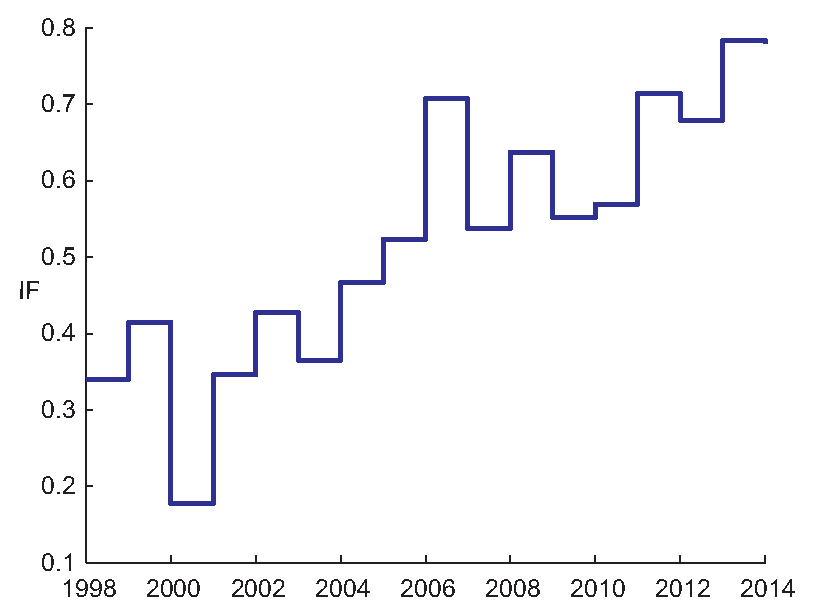
\includegraphics[width=75mm]{fig1}
\caption{Recent values of the Impact Factor (IF) of AAA as computed by
Thomson-Reuters. Please do not forget that the IF is first, a measure of
the size of a discipline.}
\label{fig1}
\end{figure}

\begin{figure}
\centering
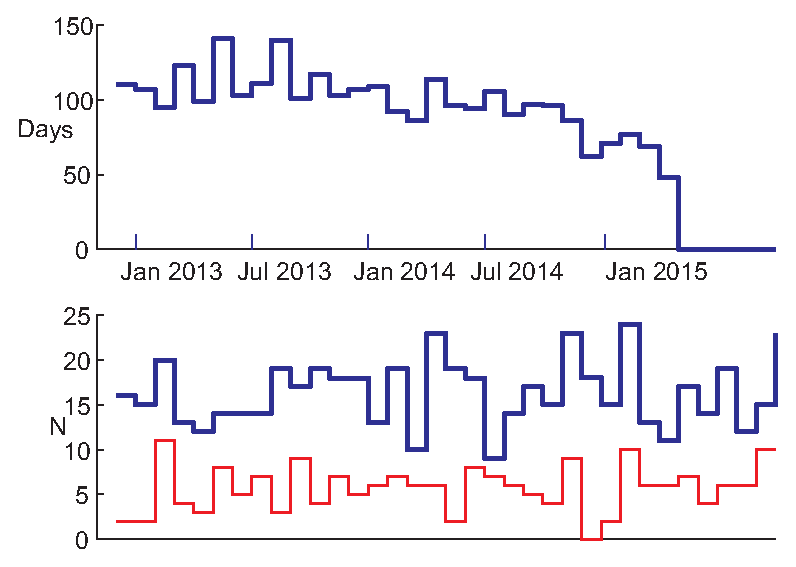
\includegraphics[width=75mm]{fig2}
\caption{(Colour online) Top: total time from first submission to first
Editor decision (in days) since 3 years. The values of the most recent
months are not significant, and have been zeroed. Both the Editorial
Board and the reviewers do their best to provide useful reviews in a
reasonably short time! Bottom: monthly number of spontaneous submission
(thick, black line); monthly number of rejected papers (thin, grey
line). }
\label{fig2}
\end{figure}

If the figures are on separate pages, the number of each figure and the
name of the first author must be marked.

Figures in the print version of the journal are usually reproduced in
black and white. Inclusion of coloured figures in the print version
requires a special fee to be paid to the publisher. In the online
version of the journal colour figures can be included at no extra cost,
provided that the information contained in them is clearly recognizable
and distinguishable when printed in black and white in the print
version. A price list is given on \\
http://www.acta-acustica-united-with-acustica.com/\\
\hspace*{24pt}for-authors/colour-reproduction-in-print.html.

When preparing illustrations that will appear in colour in the online
journal and in black and white in the print journal, authors must ensure
that the chosen colours appear suitably when printed in black and white.
Descriptions of figures in the text and captions should apply clearly to
both versions, print and online. If a figure will appear in black and
white in the print journal and in colour in the online journal, the
statement ``(Colour online)'' should be added to the figure caption. The
caption of colour figures that appear in black and white in the print
journal may not contain indications referring to colours, such as ``red
line'', ``blue line'' etc.

\subsection{Bibliography}

Articles submitted to Acta Acustica united with Acustica should cite
all relevant work, part of which should have appeared in Acoustics
journals such as Acta Acustica united with Acustica. This criterion
will be applied to determine whether the article is within scope of
the journal.

The number of citations should not exceed 80 except for review papers.
References are cited by numbers in rectangular brackets, for example
\cite{3,4}. The reference list is placed at the end of the manuscript.
The order of references is according to their appearance in the article.
All author names should be included in the reference (cf. References
below).

For Latex contributions, if the bibliography is done in an external
.bib file, authors are asked to upload both the .bib and the .bbl
files obtained by a ``bibtex'' compilation of the main .tex file
on their own computer.

The official abbreviation for Acta Acustica united with
Acustica is ``Acta Acust united Ac''.


\section{Submission}

New and revised manuscripts shall be submitted online at the EM website,
http://www.editorialmanager.com/aaa/ (see also the instruction for
authors and reviewers given by Editorial Manager). The following
information will need to be provided during submission:

\subsection{Article type}

Acta Acustica united with Acustica publishes review papers, scientific
papers, short communications, technical and applied papers, letters
to the editor, and a new article type: fast track.
\begin{description}
\item[Review Papers] discuss the state-of-the-art in an area of
      acoustics that seems of particular interest to the community at
      this point in time; review papers should be particularly complete
      in covering literature and should mention all ideas, models,
      experiments, even if they do not correspond to the authors own
      opinion. Before writing a review paper, please contact the
      Editor-in-Chief.
\item[Scientific Papers] contain original material (ideas, models,
      experiments) not published elsewhere, that contributes
      substantially to the advance of science in the field of acoustics;
      they should clearly establish the relation between the work
      reported on, and the state-of-the-art; scientific papers are
      typically not longer than 12 pages.
\item[Technical and Applied Papers] report on original applications of
      an existing technique, concept, or measurement method to a new
      area; it is essential that a technical and applied paper is of
      sufficient interest to a group of researchers and engineers beyond
      the specific application or geographic area.
\item[Short Communications] are short scientific papers typically not
      longer than 4 pages; one can use a short communication to report
      on original, new ideas, models, or experimental results, that do
      not require a substantial discussion; they are NOT scientific
      papers of poor quality.
\item[Letters to the Editor] are promoted as a forum to stimulate
      scientific discussion; typically they contain critical comments on
      or additions to published work by the author or his/her peers;
      they may also introduce new ideas for future research with
      preliminary results without the proof required for a scientific
      paper; the scientific level needs nevertheless be guaranteed.
\item[Fast Track Articles] are a new article type, which stands for fast
      peer-review, fast production of accepted manu\-scripts and
      immediate open access publication. It is for short scientific
      papers characterized by their concision and originality. The
      length is limited to 4 pages. For this article type there is a
      mandatory fast track fee due on acceptance (see Section~6.2).
\end{description}
For accepted scientific papers, technical and applied papers and review
papers there is a paid open access publication option upon acceptance of
a manuscript (alternatively to publishing a paper as a subscription
article without a publication fee) (see Section~6.1).

\subsection{Title}

The manuscript title should be chosen carefully to reflect the content
of the manuscript. No claims for novelty should appear in the title.

A short title should be suggested to appear in the heading of each page
of the article.

\subsection{Author(s) and their affiliation}

The corresponding author should be fully registered in the online
manuscript handling system. For other authors that are not registered,
entering name and affiliation is sufficient. The submitting author can
select a different author to become the corresponding author.

\subsection{Field (Section/Category)}

Manuscripts will be published and indexed under this Field in Acta
Acustica united with Acustica.

\subsection{Summary and conclusion}

The summary should be a brief and precise representation of the content
of your manuscript. The choice of wording is of utmost importance since
searching in different indexes is mainly based on the summary text. The
Summary must be limited to 200 words for Papers, or to 100 words for
Letters to the Editor and Short Communications.

The conclusion summarizes the consequences of the work. It differs from
the summary. Authors need to distinguish ``The method XXX has been
applied...'' from ``The method XXX allows to...'' or ``The method XXX is
limited by...'', for example.

\subsection{Classification (PACS number)}

For additional classification and for selecting reviewers, the PACS
(Physics and Astronomy Classification Scheme) is used. Please select one
to five keywords accurately describing the area of your manuscript from
the list.

\subsection{Statement concerning the originality of the work}

A manuscript can only be considered for publication if it is not under
review or in print with another journal, as a whole or in substantial
part. Previous submission to another journal is no objection, but the
reason for submitting to Acta Acustica united with Acustica should be
clarified.

\subsection{Comments to the Editorial Office (optional)}

Optionally, additional comments to the editorial board can be added.
These comments will not be forwarded to the reviewers.

\subsection{Suggested reviewers}

With the exception of Letters to the Editor, the author is requested to
suggest three reviewers. The editors are free to follow these
suggestions or not. Please do not suggest three reviewers from the same
country. Optionally, the author can oppose possible reviewers. Please
give a good reason to oppose a reviewer. The editors reserve the right
to ignore these objections.

\subsection{Downloading files} \label{Manuscript files and figures}

Files containing the manuscript and figures should be uploaded online.
At least one item ``Manuscript'' should be attached to the submission.
If multiple documents are added, they will be included in the
automatically generated PDF file used for review in the order given in
the submission.

Figures should be submitted as separate files (a vector graphic format
is required except for photographs). In the event of any problems while
uploading a manuscript, please contact the Editor-in-Chief's office at
the address given below.

Once the above information is entered into the system, a manuscript PDF
file will be generated. The submitting author should approve this
automatically built file. Your manuscript will then be assigned a
manuscript number and the Editor-in-Chief will forward it to an
appropriate Associate Editor. The Associate Editor will send the
manuscript to referees, supervise the reviewing process and inform you
of his/her decision. Final disposition is up to the Editor-in-Chief. You
can follow the review process at any time by logging in to the EM
website, http://www.editorialmanager.com/aaa/.


\section{Special issues}

For topics of special interest, the Editor-in-Chief can decide to
publish a special issue (or a special section in a regular issue).
Proposals should be submitted to him. The following rules apply: two
Associate Editors from two different countries are appointed; authors of
several countries are invited to submit a paper; the peer-review process
is regular; the paper format is the format of regular papers.


\section{Proofs, Copyright, self-archiving policy and Offprints}

\subsection{Proofs}

Proofs will be sent to the person indicated as the corresponding author
at submission of the manuscript on the first page of the manuscript. The
corrected proofs should be returned within 8 days; corrections should be
carefully done and clearly indicated. No new material can be inserted in
the text at the time of proof reading.

\subsection{Copyright assignment}

The corresponding author will need to fill in and sign the
{\em Copyright Transfer Statement} for the journal and return it to the
publisher. Please see this form on the journal's website for information
on what rights you retain as an author and information on the
publisher's self-archiving policy for authors, \\
http://www.acta-acustica-united-with-acustica.com/for- \\
\hspace*{24pt}authors/copyright-self-archiving-policy.html. \\
The above holds for subscription articles without a publication fee
only. For paid open access articles and fast track articles, see
Section~6.3.

\subsection{Offprints}

As soon as the article has been published in the online version of Acta
Acust united Ac a complimentary copy of the article in PDF format will
be sent to the corresponding author, together with a notification letter
recapitulating the Copyright and Self-Archiving Policy of the Journal.



\section{Open Access publication option, Fast Track Article option,
Fees} \label{OA}

\subsection{Open Access publication option for research articles}

Alternatively to publishing a paper as a subscription article without a
publication fee, there is a paid open access publication option upon
acceptance of a manuscript. Authors may choose this option, if they wish
to have their accepted manuscripts (scientific papers, technical and
applied papers, review papers) published immediately open access upon
publication without any embargo period. For instance, open access might
be a requirement of their institutions or research funders, allowing
also non-subscribers of the journal to access their articles
free-of-charge.
\begin{itemize}
\item  Upon acceptance of a manuscript authors will be asked, if they
   wish to choose paid open access publication. Five working days after
   acceptance of the manuscript and receiving the acceptance
   notification, at the latest, authors must inform the publisher, if
   they choose this option.
\item  For this option, authors, their institutions, or their research
   funders are required to pay an Article Publication Charge (APC) of
   EUR 1200 (plus VAT, if applicable).
\item  Payment can be made either directly online by credit card, or with
   a bill/invoice request.
\item  Receipt of payment is a prerequisite of publishing the article
   open access immediately upon publication of the respective issue.
\end{itemize}

\subsection{Open Access Fast Track Article}

Authors may choose this article type for fast track and open access
publication of short scientific papers characterized by their concision
and originality.
\begin{itemize}
\item  The Fast Track article type (with mandatory fast track fee upon
   acceptance) is chosen upon submission of a manuscript.
\item  The maximum length is 4 pages (two columns); otherwise the
   manuscript instructions in Section~2 apply.
\item  The submission and peer-review modalities are that of scientific
   papers; however the ``major revision'' decision does not exist; if the
   paper is not accepted, a new submission as a paper of another type is
   requested.
\item  The objective is to publish the paper online within 2 months from
   submission; the time for (minor) revisions by the authors is limited
   to 20 days.
\item  Online access to the
   article is possible before the publication of the respective journal
   issue (fast track).
\item  The paper is published in a special section at the beginning of a
   regular issue (print and online version).
\item  Fast track online access to the article is possible before and
   independent of the time schedule of the actual publication date of
   the respective journal issue.
\item  For this option, authors, their institutions, or their research
   funders are required to pay a mandatory fast track fee of EUR 450
   (plus VAT, if applicable).
\item  On acceptance of the manuscript authors are offered a choice of
   how to make payment: Payment can either be made directly by an author
   online by credit card, or with a bill/invoice request. All
   information will be given to the authors during the submission and
   acceptance process on Editorial Manager.
\item  Receipt of payment is a prerequisite of publishing the article
   fast track and open access.
\end{itemize}

\subsection{General}

\begin{itemize}
\item  All Open Access articles, including Fast Track articles, are
   subject to thorough, independent peer-review.
\item  If an author wishes to have four-colour illustrations in the print
   version, the extra costs as given under ``Section 2.3.2 Figures''
   apply. This is not covered by an APC or fast track fee.
\item  For articles to be published Open Access, the
   sub\-mitting/corresponding author needs to fill in and sign the Open
   Access Agreement available on the journal's website, see\\
   http://www.acta-acustica-united-with-acustica.com/ \\
\hspace*{24pt}fileadmin/Dateien/Open\_Access\_Agreement/ \\
\hspace*{24pt}AAuA\_Open\_Access\_Agreement.pdf
\item  For published Open Access articles, including Fast Track, and
   provided an APC or fast track fee is paid, authors are not required
   to transfer but will retain their copyright.
\item  All Open Access articles are published under a Creative Commons
   Attribution (CC BY 4.0) \\ http://creativecommons.org/licenses/by/4.0.
\item  Authors are also permitted to post the final, published PDF of
   their Open Access article on his/her own personal website, his/her
   institutional repository, his/her funder's (designated) repository or
   on any other free public server, immediately on publication. There is
   no embargo period.
\end{itemize}


\section{Addresses}

Correspondence concerning manuscript status should be directed to
the Editor-in-Chief: 
\begin{quote}
Prof. Jean Kergomard \\
 Directeur de recherche \\
 Laboratoire de Mécanique et d'Acoustique\\
 CNRS - 4 impasse Nikola Tesla CS 40006\\
 13453 Marseille Cedex 13 France\\
 E-mail: AAA@lma.cnrs-mrs.fr 
\end{quote}
Inquiries concerning manuscript style, file formats, layout of tables
and figures and of the final paper may be sent to the Production Manager: 
\begin{quote}
Dr. Johann Wempen\\
 Daucherstr. 98\\
 D-85053 Ingolstadt\\
 Phone +49 841 97 5852\\
 E-mail: wempen@t-online.de 
\end{quote}
\noindent Publisher: 
\begin{quote}
S. Hirzel Verlag\\
 Birkenwaldstr. 44\\
 70191 Stuttgart\\
 PO Box 10 10 61\\
 70009 Stuttgart\\
 Germany\\
 Phone +49 (0)711 25 82-0\\
 Fax +49 (0)711 25 82-290\\
 E-mail: ActaAcustica@Hirzel.de 
\end{quote}

\subsection*{Acknowledgement}

If appropriate.

\small
\bibliographystyle{plain}
\begin{thebibliography}{1}
\bibitem{1} F. Mittelbach, M. Goossens,J. Braams, D. Carlisle, C.
   Rowley: The LaTeX Companion. {S}econd edition. Addison-Wesley
   Professional, Bonn, Germany, 2004.
\bibitem{2} The LaTeX Project, LaTeX -- {A} document preparation
   system, www.latex-project.org, 2011.
\bibitem{3} B. C. J. Moore, Gockel: Factors influencing sequential
   stream segregation. Acta Acust united Ac \textbf{88} (2001) 320--333.
\bibitem{4} L. Cremer, H. A. M\"uller: Principles and applications
   of room acoustics. Chapman and Hall, London, 1982.
\end{thebibliography}

\end{document}

